\section{Coarse-grain Dynamic Execution}
\label{sec:course_grain}

\begin{figure}
	\centering
	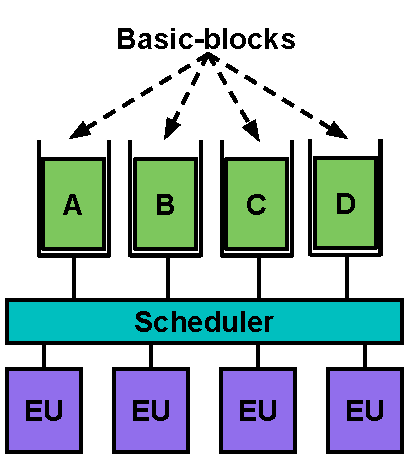
\includegraphics[width=0.5\columnwidth]{fig/coarse_grain_sch.pdf} 
	\caption{Coarse-grain execution model}
	\label{fig:coarse_grain_sch}
\end{figure}

In this work, we introduce the notion of coarse-grain execution where every
cluster of instructions is a unit of execution that is statically scheduled to
run optimally without further dynamic scheduling by the hardware. We call it the
{\it{Phraseblock}}. Phraseblock differs from other instruction clustering
definitions such as superblocks~\cite{superblock} and
hyperblocks~\cite{hyperblock} in that its purpose is to group the set of
instructions that, ideally, can execute without an unpredictable latency
interruption. 

The simplest form of a phraseblock is the program basic-block whose energy and
performance are evaluated in this work. Similar to an instruction, the
basic-block is a single-entry, single-exit unit without any control stalls.
Memory stalls are possible within a basic-block, but with effective static
scheduling, their impact on stalling other independent instructions in the
basic-block is minimized.

In the presence of unpredictable memory and control stalls, a fully static
schedule cannot deliver the same code quality as a dynamic scheduler like the
Tomosulo's algorithm~\cite{tomasulo}. To address the problem with unpredictable
long latency operations, we combine static and dynamic scheduling to leverage
static scheduling for saving energy while delivering optimal code schedules, and
to leverage dynamic scheduling only for hiding unpredictable long latency events
such as cache misses. To do so, we allow multiple speculative basic-blocks to be
in-flight at the same time to dynamically contend for resources.  Each
basic-block is statically scheduled and issues its instructions in-order.  As a
result, when a load operation in a basic-block misses in the L1, it stalls,
    though other in-flight basic-blocks issue instructions to hide its latency.
    Figure~\ref{fig:coarse_grain_sch} illustrates four basic-blocks placed in
    four first-in-first-out (FIFO) instruction queues, contending to schedule
    their instructions on one of the available execution units (EU).
